\documentclass[10pt, a4paper]{scrartcl}

\usepackage{vorschule}
\usepackage[
    typ=ab,
    fach=Mathematik,
    lerngruppe={Q1 GK},
    nummer=17,
    module={Symbole,Lizenzen},
    seitenzahlen=keine,
    farbig,
    lizenz=cc-by-nc-sa-4,
]{schule}

\usepackage[
	kuerzel={Ngb},
	reihe={Analysis III},
	version={2019-03-31},
]{ngbschule}

\author{J. Neugebauer}
\title{Eine besondere Exponentialfunktion}
\date{\Heute}

\usepackage{tinspire}

\setzeAufgabentemplate{ngbnormal}
%\setzeAufgabentemplate{schule-binnen}

\begin{document}
	\ReiheTitel
	
	Viele Wachstumsprozesse verlaufen \emph{Exponential} und können mathematisch 
	mit einer \emph{Exponentialfunktion} modelliert werden. Eine allgemeine 
	Exponentialfunktion hat die Form
	\[ f(x) = a\cdot b^x \]
	
	Für den Fall $a = 1$ und abhängig von der Basis $b$ lässt sich mit Hilfe des \emph{Differenzenquotienten} die
	Ableitung bestimmen:
	\[ f_b(x) = b^x \qquad f_b'(x) = f_b'(0)\cdot b^x \]

	Für die Basis $b = 2$ sieht der Graph der Funktion und ihrer Ableitung beispielsweise so aus:
	\begin{center}
		\begin{tikzpicture}[scale=.6]
		\tkzInit[xmin=-5,xmax=5,ymin=0,ymax=8]
		\tkzGrid[color=gray!20]
		\tkzAxeXY[origin=false,font=\sffamily\tiny]
		\tkzFct[color=NavyBlue,line width=1pt]{2 ** x}
		\tkzFct[color=NavyBlue,line width=1pt,style=dashed]{0.693 * 2 ** x}
		
		\tkzDefPoint[label=above:$f_2(x)$](1,3){A}
		\tkzDefPoint[label=right:$f_2'(x)$](2,2){B}
		\end{tikzpicture}
	\end{center}

	\begin{aufgabe}
		Beschreiben sie Besonderheiten der Ableitungsfunktion $f_b'(x)$. Was ist sie für eine Art Funktion und wie ist sie definiert?
	\end{aufgabe}

	\begin{aufgabe}
		Untersuchen sie die Exponentialfunktion mit dem Taschenrechner. Befolgen sie dazu zunächst die Anleitung auf der Rückseite, um ein neues Dokument zu erstellen. Stellen sie dann verschiedene Werte für die Basis ein.
		
		Was fällt ihnen auf? Notieren sie Basen (Werte für $b$), die ihnen besonders erscheinen.
	\end{aufgabe}

	\begin{aufgabe}[symbol=\symStern]
		Erinnern sie sich: Welche Eigenschaften haben alle Exponentialfunktionen?
		
		Zum Beispiel:
		\begin{itemize}
			\item Durch welche Punkte verlaufen sie?
			\item Wann wachsen / wann fallen sie?
			\item Welchen \emph{Startwert} haben sie?
		\end{itemize}
	
		Nutzen sie ihre Formelsammlung, um ihr Gedächtnis zu 
		unterstützen.
	\end{aufgabe}

	\newpage
	\textbf{Exponentialfunktion im \TIN untersuchen}\\
%	\begin{multicols}{2}
		\begin{enumerate}
			\item Rufen sie das Dashboard mit \TINon* auf und erstellen sie ein neues Dokument mit \TINnum{1} (speichern sie ggf. ihr aktuelles Dokument).
			\item Fügen sie ein Graphen-Blatt mit \TINnum{2} ein (\texttin{2:Graphs hinzufügen}).
			\item Die Eingabezeile für eine Funktion sollte nun offen sein und auf eine Eingabe warten ($f1(x)=$). Ist dies nicht der Fall, können sie mit \TINtab die Eingabezeile öffnen.
			\item Geben sie die Formel der allgemeinen Exponentialfunktion ein ($f1(x) = b^x$) und bestätigen sie mit \TINenter*.
			\item Das Dialogfenster \enquote{Schieberegler erstellen} bestätigen sie wieder mit \TINenter*.
			\item Sobald das Eingabefenster geschlossen ist wechseln sie mit \TINtab wieder in die Eingabezeile. Drücken sie die Taste rechts neben der \TINnum{9} und finden sie das Symbol für die Ableitung ($\tfrac{d}{d\square}\square$). Ergänzen sie die Eingabezeile zu $f2(x) = \tfrac{d}{dx}(f1(x))$ und bestätigen sie wieder mit \TINenter*.
			
			Der Graph der Funktion $f2$ stellt nun die Ableitung der Funktion $f1$ dar.
			\item Bewegen sie den Zeiger mit dem Trackpad über den Schieberegler und drücken sie \TINctrl + \TINmenu*. Wählen sie im Menü \texttin{2:Einstellungen...}.
			\item Konfigurieren sie den Schieberegeler wie gezeigt:
				\begin{center}
					\begin{tinwindow}{Schiebereinstellungen} 
						\TINwfield[1]{Anfangswert:}
						\TINwfield[1]{Minimum:}
						\TINwfield[5]{Maximum:}
						\TINwfield[0.2]{Schrittweite:}
					\end{tinwindow}
				\end{center}
			\item Durch einen Druck auf den Pfeil nach rechts wird der \texttt{OK} Knopf ausgewählt und mit \TINenter* das Fenster geschlossen werden.
			\item Mit dem Zeiger können sie nun den Schieberegler verschieben und die Veränderung der Graphen beobachten. 
			
			Passen sie ggf. noch den Zoombereich an, um einen besseren Ausschnitt zu sehen.
		\end{enumerate}
%	\end{multicols}
	
\end{document}